\documentclass[12pt,a4paper]{scrartcl}

% die folgenden Packete erlauben den Gebrauch von Umlauten und ß
%
%  German quotes
%
\newcommand{\qq}[1]{\glqq{}#1\grqq{}}
%
%  absolute value, norms
%
\newcommand{\abs}[1]{\left | #1 \right |}
\newcommand{\norm}[1]{\left \| #1 \right \|}
\newcommand{\twonorm}[1]{\left \| #1 \right \|_2}
\newcommand{\supnorm}[1]{\left \| #1 \right \|_\infty}
%
%
\newcommand{\hhalbe}{ \frac{h}{2} }
\newcommand{\hviertel}{ \frac{h}{4} }
%
% in der Latex Datei
%\usepackage[utf8]{inputenc}
\usepackage[latin1]{inputenc} %  Alternativ unter Windows
\usepackage[T1]{fontenc}
% \usepackage[ngerman]{babel}
% This time i write in english
\usepackage[english]{babel}

\hyphenation{po-si-tive}
\hyphenation{equi-va-lent}
\hyphenation{ne-ces-sary}
\hyphenation{pro-ba-bi-li-ty}

\usepackage{pgfplots}

%\usepackage[pdftex]{graphicx}
\usepackage{latexsym}
\usepackage{mathtools}
\usepackage{amssymb,amsthm}
%\usepackage{amsmath,amssymb,amsthm}
%\allowdisplaybreaks

\usepackage{enumerate}
\usepackage{multirow}

%\usepackage[Algorithmus]{algorithm}
%\usepackage{algpseudocode}

%\restylefloat{figure}		% ermoeglicht option [H] (only HERE!)
\usepackage{float}
\usepackage{subfigure}
%\usepackage{subcaption}

\usepackage{tikz}
\usetikzlibrary{arrows}

% useful packages
\usepackage[linktoc=section]{hyperref}
\usepackage[colorinlistoftodos, disable]{todonotes}	% if you want to disable all todos, use the option 'disable'!

%\floatstyle{plain}

% Abstand obere Blattkante zur Kopfzeile ist 2.54cm - 15mm
\setlength{\topmargin}{-15mm}


% some abbreviations
\newcommand{\ul}[1]{\underline{#1}}
\newcommand{\ol}[1]{\overline{#1}}

\newcommand{\C}{\mathbb{C}} % komplexe
\newcommand{\K}{\mathbb{K}} % bel. Koerper
\newcommand{\R}{\mathbb{R}} % reelle
\newcommand{\Q}{\mathbb{Q}} % rationale
\newcommand{\Z}{\mathbb{Z}} % ganze
\newcommand{\N}{\mathbb{N}} % natuerliche

\newcommand{\PP}{\mathbb{P}} % Wahrscheinlichkeitsmaß P
\newcommand{\E}{\mathbb{E}} % Erwartungswert

\newcommand{\mc}[1]{\mathcal{#1}}	% kaligraphisch shortcut

\newcommand{\dx}{\,\mathrm{d}x}
\newcommand{\da}{\,\mathrm{d}a}
\newcommand{\ds}{\,\mathrm{d}s}
\newcommand{\dt}{\,\mathrm{d}t}

\newcommand{\rhoIn}{\rho_{\text{in}}}
\newcommand{\GammaIn}{\Gamma_{\text{in}}}

\newcommand{\FigureHSpace}{\hspace*{-1.0em}}

%% genetic Algorithms - Start
\newcommand{\ff}{\mathit{ff}}
%% genetic Algorithms - Ende
%
%% Mathematische Operatoren
\DeclareMathOperator{\DIV}{div}
\DeclareMathOperator{\SPAN}{span}
\DeclareMathOperator{\SUPP}{supp}
\DeclareMathOperator{\ID}{id}
\DeclareMathOperator{\ROUND}{round}
%

% Change \part header.
\usepackage{titlesec}
%\usepackage{titletoc}
%\renewcommand{\part}[1]{\paragraph{#1}}
%\addto\captionsenglish{\renewcommand{\partname}{Sthg else}}
\titleformat{\part}[hang]{\bfseries\Huge}{\thepart.}{0.5em}{}
\renewcommand{\thesection}{\arabic{section}.}
\renewcommand{\thesubsection}{\arabic{section}.\arabic{subsection}.}
\renewcommand{\thesubsubsection}{\arabic{section}.\arabic{subsection}.\arabic{subsubsection}.}

% Change equation labelling to default.
\renewcommand\theequation{\thesection\arabic{equation}}


%% Start section numbering new after a new part
\makeatletter
\@addtoreset{section}{part}
\makeatother


\begin{document}

% Keine Seitenzahlen im Vorspann
  \pagestyle{empty}

  % Titelblatt der Arbeit
  \begin{titlepage}

%    \includegraphics[scale=0.45]{kit-logo.jpg} \hfill \includegraphics[scale=0.15]{mathe-logo.jpg}
    \vspace*{2cm}

	 \begin{center} \large

    Lecture Notes\\
    %---\\
    %Übungsblatt 1, 2
    \vspace*{2cm}

    {\huge \ Artificial Intelligence}
    \vspace*{2.0cm}

    Michael Maier \\
    \vspace*{1.5cm}

    Wintersemester 2015/2016
    \vspace*{2.8cm}


    %Betreuung: Johannes Ernesti und Ramin Shirazi-Nejad \\[1cm]
    %Fakultät für Mathematik \\[1cm]
	%	Karlsruher Institut für Technologie
	Lecturer: Dr Piotr Prokopowicz \\[1cm]
   Faculty of Mathematics, Physics \& Technical Sciences \\[1cm]
		Kazimierz Wielki University

 	\end{center}
 \end{titlepage}


% Inhaltsverzeichnis
\tableofcontents


  % Ab sofort Seitenzahlen in der Kopfzeile anzeigen
  \pagestyle{headings}

\newpage

%%%%%%%%%%%%%%%%%%%%%%%%%%%%%%%%%
%%%%%%%%%%% CONTENT %%%%%%%%%%%%%
%%%%%%%%%%%%%%%%%%%%%%%%%%%%%%%%%


%%%%%%%%%%% Fuzzy Logic %%%%%%%%%%%%
\part{Fuzzy Systems}

%%%%% Content %%%%%

In normal Logic we only differentiate if a statement is true or false. But if we want to model the real world, there are some statements which cannot clearly be decided as true or false, e.g. the car is comfortable or the car is old. This can be modelled by fuzzy sets.


%%% §1 %%%
\section{Fuzzy Sets}
In regular crisp set theory an element $x$ of a (crisp) set $\Omega$ either belongs to a (crisp) subset $A$ or not. In Fuzzy Logic we define a (membership) value $\ol A(x)\in[0,1]$ for an element $x\in\Omega$, which describes the membership of $x$ to a subset $A$. So in case of a crisp set $A$ we have $\ol A(x)=1$ if $x\in A$ and if $x\notin A$, then $\ol A(x)=0$.

\subsection{Knowledge Representation in a fuzzy set}
In normal speech the age of a person is not always described with the exact age, mostly some description as \emph{young}, \emph{old}, \emph{around 40} or \emph{between 30 and 40} is used. \\
This should be modelled by fuzzy set theory too, so a fuzzy set should not only model numerical variables, it should also be able to model linguistic variables like \emph{age}, \emph{speed} or \emph{temperature}, \qq{whose (linguistic) values are words or sentences in a natural or artificial language}\cite{IntrFuzzyControl}. \\
Therefore a fuzzy set can contain different types of elements:
\begin{itemize}
\item Real Numbers,
\item Fuzzy Numbers (e.g. \emph{approximately 4} or \emph{(approximately) between 3 and 4}; see \ref{sec:fuzzyNumbers}),
\item Linguistic values (e.g. \emph{large}, \emph{very large}, \emph{old}, \emph{young}, \emph{pretty} or \emph{nice}; see \ref{sec:linguicVar}).
\end{itemize}


\subsubsection{Linguistic Variables and Values} \label{sec:linguicVar}
As mentioned above, linguistic variables are described by linguistic values. But for the calculation with linguistic variables we need some numerical representation or information of the linguistic values.\\
Therefore a linguistic variable is associated with the following notion:
\[ \langle X,\mc LX, \mc X, M_X \rangle, \]
where:
\begin{itemize}
\item[$X$] is the \emph{symbolic name} of the linguistic variable (e.g. age, speed or temperature)
\item[$\mc LX$] is the \emph{set of linguistic values} (also \emph{term-set}, \emph{reference-set}), that $X$ can take (e.g. young, middle, old for age or (very) slow, normal, (very) fast for speed)
\item[$\mc X$] is the \emph{physical domain} (also \emph{universe of discourse}) over which the (linguistic) variable $X$ takes its quantitative (crisp) values (e.g. the interval $[0$ km/h, $400$ km/h $]$ for speed)
\item[$M_X$] is a \emph{semantic function} that refers to every element (linguistic value) $LX\in\mc LX$ a physical, so quantitive, meaning or interpretation. This meaning/interpretation is represented by a fuzzy set $\widehat{LX}$, that is defined over $\mc X$ (e.g. a car is fast if it drives (at least) approximately $100$ km/h, see \ref{sec:fuzzyNumbers} for a possible fuzzy number that models this). Ofttimes also the membership function $\mu_{LX}:=M_X(LX)$ is used.
\end{itemize}
As an example, we can define a fuzzy (sub-)set $\ol A$ of $\{ very\, small, small, medium, high, very\, high \}$ that models e.g. the height of trees:
\[ \ol A(small)=0.3,\quad \ol A(medium)=1.0, \quad \ol A(high)=0.7. \]
$\ol A$ is a \textbf{discrete fuzzy set} and is commonly written as
\[ \ol A = \left\{ \frac{0.3}{small}, \frac{1.0}{medium}, \frac{0.7}{high} \right\}. \]
For this example we then can define the linguistic variable $X=H:=$ \textit{height (of trees)}, term-set $\mc LH=\{ very\, small, small, medium, high, very\, high \}$, universe of discourse $\mc H=[0$ m, $60$ m$]$ and the semantic/membership function $M_H$, respectively $\mu_{LH}$, defined as following:
\begin{align*}
\mu_{small}(x) = M_H(small)(x) :=& \ \begin{cases}
		1, &x \leq 8 \\
		\frac{16-x}{8}, &8 < x < 16 \\
		0, &x \geq 16
	\end{cases} \\
	 \widehat{=}& \quad \qq{\text{height is less than $16$m.}} \\
\mu_{medium}(x) = M_H(medium)(x) :=& \ \begin{cases}
		0, &x \leq 8 \\
		\frac{x-8}{8}, & 8 < x < 16 \\
		1, &x = 16 \\
		\frac{24-x}{8}, &16 < x < 24 \\
		0, &x \geq 24
	\end{cases} \\
	\widehat{=}& \quad \qq{\text{height is about $16$m.}} \\
\mu_{high}(x) = M_H(high)(x) :=& \ \begin{cases}
		0, &x \leq 16 \\
		\frac{x-16}{8}, &16 < x < 24 \\
		1, &x \geq 24
	\end{cases} \\
	\widehat{=}& \quad \qq{\text{height is more than $16$m.}}
\end{align*}
$\mu_{small},\, \mu_{medium}$ and $\mu_{high}$ are socalled \emph{fuzzy numbers} (\ref{sec:fuzzyNumbers})  and can be illustrated as following:
\begin{figure}[H]
\centering
\begin{tikzpicture}
	\begin{axis}[grid=both,ymin=-0.25,ymax=1.25,xmin=4,xmax=28,
               minor tick num=1,
               %axis lines = middle,
               xlabel=\text{height [m]},ylabel=\text{membership value},
               %legend style={at={(axis cs:40,0.5)},anchor=east}
               ]
		% add line "small"\\
		%\addlegendentry{small}
		\addplot [mark=none,green,thick] coordinates { (4,1) (8,1) (16,0) (45,0) } node [pos=0.01,above right] {small};
		% add line "medium"
		%\addlegendentry{medium}
		\addplot [mark=none,blue,thick] coordinates { (4,0) (8,0) (16,1) (24,0) (45,0) } node [pos=0.295,above] {medium};
		% add line "high"
		%\addlegendentry{high}
		\addplot [mark=none,red,thick] coordinates { (4,0) (16,0) (24,1) (45,1) }node [pos=0.57,above left] {high};
  \end{axis}
\end{tikzpicture}
\end{figure} \FigureHSpace
Therefore the linguistic variable \textit{height} is in our case associated with this notion:
\[ \langle H, \mc LH, \mc H, M_H \rangle = \langle height, \{ very\, small, small, medium, high, very\, high \}, [0,60], M_H \rangle.\]

\subsection{Arithmetic of fuzzy sets} \label{sec:fuzzyArithm}
As in the regular sets theory we want to define the intersection $\ol A\cap\ol B$, the union $\ol A\cup\ol B$ and the complement $\ol A^c$ of $\ol A$:\\
The \emph{complement} is defined via the membership-function
\[ \ol A^c(x) = 1-\ol A(x). \]
The \emph{intersection} for fuzzy sets $\ol A,\ol B$ defined on the same support $X:=\SUPP(\ol A)=\SUPP(\ol B)$ can be defined by ($x\in X$)
\[ (\ol A\cap\ol B)(x) = T(\ol A(x),\ol B(x)), \]
for a so-called \emph{t-norm} $T$, that has the following specifications ($x\in X$):
\begin{enumerate}[1)]
\item $T(\ol A(x),1)=\ol A(x)$
\item $T(\ol A(x),\ol B(x))=T(\ol B(x),\ol A(x))$ (Symmetry)
\item if $\ol B_1(x)\leq \ol B_2(x)$, then $T(\ol A(x),\ol B_1(x))\leq T(\ol A(x),\ol B_2(x))$ (Monotony)
\item $T(\ol A(x),T(\ol B(x),\ol C(x)))=T(T(\ol A(x),\ol B(x)),\ol C(x))$ (Associative)
\end{enumerate}
Note that $T(1,1)=1, T(0,1)=T(1,0)=T(0,0)=0$, so if it is reduced to crisp sets we obtain exactly the intersection $A\cap B$ for crisp sets.\\
Similar as above, the \emph{union} for fuzzy sets $\ol A,\ol B$ defined on the same support $X:=\SUPP(\ol A)=\SUPP(\ol B)$ can be defined by ($x\in X$)
\[ (\ol A\cup\ol B)(x) = C(\ol A(x),\ol B(x)), \]
for a so-called \emph{t-conorm} $C$, that has the following specifications:
($x\in X$)
\begin{enumerate}[1)]
\item $C(\ol A(x),0)=\ol A(x)$
\item $C(\ol A(x),\ol B(x))=C(\ol B(x),\ol A(x))$ (Symmetry)
\item if $\ol B_1(x)\leq \ol B_2(x)$, then $C(\ol A(x),\ol B_1(x))\leq C(\ol A(x),\ol B_2(x))$ (Montony)
\item $C(\ol A(x),C(\ol B(x),\ol C(x)))=C(C(\ol A(x),\ol B(x)),\ol C(x))$ (Associative)
\end{enumerate}
Note that $C(1,1)=C(0,1)=C(1,0)=1, C(0,0)=0$, so if it is reduced to crisp sets we obtain exactly the union $A\cup B$ for crisp sets.


\subsubsection*{Cylindrical Extension} \label{sec:cylindExt}
If the support of $\ol A$ and $\ol B$ is not the same (e.g. $\ol A$ and $\ol B$ are describing different aspects like age and speed of cars), the \emph{cylindrical extension} is a possibility to obtain the intersection/union:\\
The idea of the cylindrial extension is to define a fuzzy relation between the fuzzy sets $\ol A$ and $\ol B$. Therefore we define extensions $\ol A^*$ and $\ol B^*$ that are defined on $\SUPP(\ol A)\times\SUPP(\ol B)$:
\[ A^*(x_1,x_2) = A(x_1), \quad \forall x_2\in\SUPP(\ol B),x_1\in\SUPP(\ol A) \]
and
\[ B^*(x_1,x_2) = B(x_2), \quad \forall x_1\in\SUPP(\ol A),x_2\in\SUPP(\ol B) \]
Now we can calculate the resulting $\ol C_{inter} = \ol A^*\cap\ol B^*$ and $\ol C_{union} = \ol A^*\cup\ol B^*$ on $\SUPP(\ol A)\times\SUPP(\ol B)$ with an intersection- and union-operator.

\vspace*{0.75cm} \hspace*{-1.5em}
With these definitions of a t-norm and t-conorm we can obtain (at least most of) the rules of regular sets theory for fuzzy sets (without proof):
\begin{itemize}
\item Idempotency,
\item Commutativity (respect to $\cup, \cap$),
\item Associativity (respect to $\cup, \cap$),
\item Absorption,
\item Distributivity,
\item Identity,
\item Law of Contradiction,
\item Law of Excluded Middle,
\item Involution,
\item De Morgan laws.
\end{itemize}
Examples of t-norms are (on a set $X=X_1\times X_2$, where $A$ is defined on $X_1$, $B$ on $X_2$ and $(x,y)\in X_1\times X_2$):
\begin{itemize}
\item Standard intersection:
	\[ T_m(\ol A(x),\ol B(y)) = \min(\ol A(x),\ol B(y)) \]
\item Bounded sum:
	\[ T_b(\ol A(x),\ol B(y)) = \max(0, \ol A(x)+\ol B(y)-1) \]
\item Algebraic product:
	\[ T_p(\ol A(x),\ol B(y)) = \ol A(x)\cdot\ol B(y) \]
\item Drastic intersection:
	\[ T^*(\ol A(x),\ol B(y)) = \begin{cases}
	\ol A(x), &\text{if } \ol B(y)=1,\\
	\ol B(y), &\text{if } \ol A(x)=1,\\
	0, \text{otherwise}
	\end{cases} \]
\end{itemize}
The advantage of $T_m$ is the fast and easy calculation, but there's no difference in the intersection if $\ol A_1(x)>\ol A_2(x)>\ol B(x)$, so we lose information about $\ol A$ (resp. $\ol A_1,\ol A_2$), since only the value $\ol B(x)$ will be used. Therefore $T_p$ is sometimes better since the information from both fuzzy sets will be used. But the choice of the intersection-operator is dependent on the application.\\
It states (for better readability without arguments):
	\[ T^* \leq T_b \leq T_p \leq T_m,\text{ in fact: } T^* \leq T \leq T_m,\quad\forall\, t\text{-norms } T. \]
Examples of t-conorms are (on a set $X=X_1\times X_2$, where $A$ is defined on $X_1$, $B$ on $X_2$ and  $(x,y)\in X_1\times X_2$):
\begin{itemize}
\item Standard union:
	\[ C_m(\ol A(x),\ol B(y)) = \max(\ol A(x),\ol B(y)) \]
\item Bounded sum:
	\[ C_b(\ol A(x),\ol B(y)) = \min(1, \ol A(x)+\ol B(y)) \]
\item Algebraic sum:
	\[ C_p(\ol A(x),\ol B(y)) = \ol A(x)+\ol B(y) - \ol A(x)\cdot\ol B(y) \]
\item Drastic union:
	\[ C^*(\ol A(x),\ol B(y)) = \begin{cases}
	\ol A(x), &\text{if } \ol B(y)=0,\\
	\ol B(y), &\text{if } \ol A(x)=0,\\
	1, \text{otherwise}
	\end{cases} \]
\end{itemize}
As with t-norms the choice of the union-operator is dependent on the application.\\
It states (for better readability without arguments):
\[ C_m \leq C_p \leq C_b \leq C^* \text{ in fact: } C_m \leq C \leq C^*,\quad\forall\, t\text{-conorms } C. \]

$T$ and $C$ are called \emph{dual} $:\Leftrightarrow$ $\begin{cases}
T(\ol A(x),\ol B(y)) = 1 - C(1-\ol A(x), 1-\ol B(y)) \\
C(\ol A(x),\ol B(y)) = 1 - T(1-\ol A(x), 1-\ol B(y))
\end{cases}$.


\subsection{Logical Rules} \label{sec:logicRules}
In this part we want to calculate logical connections between fuzzy statements like
\begin{center}
IF ( (a car is older than 30 years) AND (a car is fast) ) THEN (a car is expensive).
\end{center}
or
\begin{center}
IF ( (a car is older than 30 years) OR (a car is fast) ) THEN (a car is expensive).
\end{center}
In part \ref{sec:fuzzyArithm} we learned amongst building the complement how to intersect and unite fuzzy sets. Therefore by identifying the complement with the negation $\neg$, union with OR, intersection with AND, $\emptyset$ with $0$ and the \emph{support $X$} with $1$ we get a connection between calculations of fuzzy sets and fuzzy logic. For a complete logical model we also need the implication, which we will derive in this chapter. To clarify we show the connection between fuzzy sets and fuzzy logic with the examplary statements above: \\
If we have the fuzzy set $\ol A_1$ of cars older than 30 years and the fuzzy set $\ol A_2$ of fast cars and want to calculate the set $\ol B$ of fast cars that are older than 30 years, we obtain this via
\[ \ol B = \ol A_1\cap\ol A_2. \]
Respectively, if we want to compute the (fuzzy) set $\ol C$ of fast cars or cars older than 30 years, we get
\[ \ol C = \ol A_1\cup\ol A_2. \]
The resulting set is hereby dependent on the choice of the intersection- resp. the union-operator (compare \ref{sec:fuzzyArithm}).\\
For the implication we can make use of the following fact (let $p,q$ be statements):
\[ \text{IF } p \text{ THEN } q \Leftrightarrow \neg p \text{ OR } q \]
Then we can calculate the \emph{fuzzy implication} $\ol A\rightarrow\ol B$ with support $X_1\times X_2$ as following:
\[ (\ol A\rightarrow\ol B)(x,y) = C(1-\ol A(x), \ol B(y)), \quad (x,y)\in X_1\times X_2 \]
with a t-norm $C$, e.g. $C_m$:
\[ (\ol A\rightarrow\ol B)(x,y) = max(1-\ol A(x), \ol B(y)), \]
Another common implication operator is the \emph{Mamdani implication operator}:
\[ (\ol A\rightarrow\ol B)(x,y) = \min(\ol A(x), \ol B(y)).\]
It is based on the assumption that the truth-value of the conclusion $\ol B(y)$ cannot be higher than the truth-value of the premise $\ol A(x)$.


\subsection{Fuzzy Numbers} \label{sec:fuzzyNumbers}
Fuzzy numbers are special fuzzy sets. They express e.g. approximately a (crisp) number, an interval of the real numbers or just values \qq{(much) bigger/smaller than} a real value (compare \ref{sec:linguicVar}). \\
From \cite{IntrFuzzyLogic} we obtain the following definition of fuzzy numbers:

A fuzzy number $\ol N$ is a fuzzy subset of $\R$ with following restrictions:
\begin{enumerate}[(i)]
\item The core of $\ol N$ is non-empty ($\Leftrightarrow \exists x: \ol N(x)=1$).
\item $\alpha$-Cuts of $\ol N$ (explained in the following section) are all closed and bounded intervals.
\item The support $\{ x | \ol N(x)>0 \}$ of $\ol N$ is bounded.
\end{enumerate}
Since the core of $\ol N$ should be non-empty, $\ol N$ must be a normal fuzzy set, that means there is at least one $x$, such that $\ol N(x)=1$.


%\cite{SimulatingFuzzySystems}
\subsubsection*{Special Case}
A special case of fuzzy numbers are \emph{triangular} or \emph{triangular shaped} fuzzy numbers. They are defined by three numbers $a<b<c$, where the positive values of the fuzzy number are in the interval $(a,c)$ and the maximum value $1$ is at point $b$.\\
A \emph{triangular} fuzzy number has linear connection lines between $\ol N(a)$ to $\ol N(b)(=1)$ and from $\ol N(b)$ to $\ol N(c)$. For such a fuzzy number we write $\ol N=(a/b/c)$.\\
A \emph{triangular shaped} fuzzy number has to be continuous (or rather the graph of $\ol N$), monotonically increasing on $[a,b]$ and monotonically decreasing on $[b,c]$. We denote such a fuzzy number as $\ol N\approx (a/b/c)$.

Besides the triangular (shaped) fuzzy numbers, there is another big set of common fuzzy numbers: \emph{trapezoidal (shaped)}. They are described via $\ol T=(a/b,c/d)$ and it states: $\ol T([b,c])=\{1\}$. As the triangular (shaped) fuzzy numbers they have the same monotoneous requirements.

%\cite{IntrFuzzyLogic}
As an example, a triangular shaped fuzzy number $(1/2/3)$ is expressing \emph{approximately $2$}, a fuzzy interval $(1.5/3,5/6.5)$ is expressing a number \emph{approximately between $3$ and $5$}:
\begin{figure}[H]
\centering
\begin{tikzpicture}
	\begin{axis}[grid=both,ymin=-0.25,ymax=1.25,xmin=0,xmax=8,
               minor tick num=1,
               %axis lines = middle,
               %xlabel=\text{height [m]},
               %ylabel=\text{},
               %legend style={at={(axis cs:40,0.5)},anchor=east}
               ]
		% add line
		%\addlegendentry{small}
		\addplot [mark=none,blue,thick] coordinates { (0,0) (1,0) (2,1) (3,0) (8,0) } node [pos=0.275, above] {$(1/2/3)$};
		% add line
		%\addlegendentry{medium}
		\addplot [mark=none,red,thick] coordinates { (0,0) (1.5,0) (3,1) (5,1) (6.5,0) (8,0) } node [pos=0.5, above right] {$(1.5/3,5/6.5)$};
  \end{axis}
\end{tikzpicture}
\end{figure} \FigureHSpace

\subsubsection{$\alpha$-Cuts} \label{sec:alphaCuts}
An $\alpha$-Cut $\ol A[\alpha]$ of a fuzzy number $\ol A$ with $\ol A>0$ on $[a,c]$ is defined by:
\[ \ol A[\alpha] := \{ x\in\Omega | \ol A(x)\geq\alpha \}\subset[a,c] \quad \forall\alpha\in(0,1] \]
\[ \ol A[0] := [a,c]. \]
$\ol A[0]$ is called the \emph{support or base of $\ol A$}.\\
$\ol A[1]$ is called the \emph{core of $\ol A$}.\\
So for a triangular or triangular shaped fuzzy number $\ol N=(a/b/c)$ we obtain $\ol N[1]=\{b\}$ and %\cite{SimulatingFuzzySystems}
for a trapezoidal (shaped) fuzzy number $\ol N=(a/b,c/d)$ we get $\ol N[1]=[b,c]$.

We also know (without proof) that an $\alpha$-Cut $\ol Q[\alpha]$ for a fuzzy number $\ol Q$
is a closed and bounded interval ($0\leq\alpha\leq 1$):
\[ \ol Q[\alpha]=[q_1(\alpha), q_2(\alpha)], \]
where $q_1(\alpha)$ is an increasing, $q_2(\alpha)$ a decreasing function of $\alpha$ and $q_1(1)=q_2(1)$.


\subsubsection{Fuzzy Arithmetic}
There are two (\todo{why?}{equivalent}; without proof) ways of adding, subtracting, multiplying and dividing two fuzzy numbers:\\
\begin{itemize}
\item \todo{explain better: Norms $T$...}{Extension principle}: For $\ol C:=\ol A \ast \ol B,\quad \ast\in\{+,-,\cdot,/ \}$ we define:
	\[ \ol C:=\sup_{x,y} \{ \min(\ol A(x),\ol B(y))\, |\, x\ast y=z \} \]
	%Here the \emph{standard intersection $t$-norm} $T_m(a,b)=\min(a,b)$ was used for the extension principle (extension of the universe of discours). (compare \ref{sec:fuzzyArithm})
\item \todo{explain more?}{Interval Arithmetic/$\alpha$-Cuts}: For $\ol C:=\ol A \ast \ol B \quad\ast\in\{+,-,\cdot,/ \}$ we define:
	\[ \ol C[\alpha]:=\ol A[\alpha] \ast \ol B[\alpha] \]
\end{itemize}


%Let $\ol A,\ol B$ bew two fuzzy subsets of a set $\Omega$. Then we define:
%\begin{align*}
%\ol A\leq\ol B \quad &:\Leftrightarrow \ol A(x)\leq\ol B(x), \forall x\in\Omega\quad (\ol A \text{ is a fuzzy subset of } \ol B) \\
%\ol A<\ol B \quad &:\Leftrightarrow \ol A(x)<\ol B(x),\quad \forall x\in\Omega \quad(??\text{ or is it }\forall x\in support(\ol A)\cap support(\ol B) ??)
%\end{align*}


\subsubsection{Ordering fuzzy numbers}
Since we have a total ordering $(<,\leq,=)$ on the real numbers, we would like to have such a total ordering on the fuzzy numbers (as an extension of the real numbers) too, or at least a partial ordering (meaning: $\ol A\geq\ol B$ or $\ol A\leq\ol B$ not for all fuzzy numbers $\ol A,\ol B$).
For $\delta\in\R$ and a fuzzy number $\ol N=(a/b/c)$ or $\ol N\approx(a/b/c)$ we write $\ol N\geq(>)\,\delta$ if $a\geq(>)\,\delta$ and $\ol N\leq(<)\,\delta$ if $c\leq(<)\,\delta$.

There are a few definitions of $(<,\leq,\approx/=)$ between fuzzy numbers, but not all fulfilling the axioms of a total ordering (partial ordering: without point 4):
\begin{enumerate}[1.]
\item reflexive
\item transitive
\item $\ol M\leq\ol N$ and $\ol M\leq\ol N\, \Rightarrow\, \ol M\approx\ol N$
\item $\ol M\leq\ol N$ or $\ol M\leq\ol N\quad \forall \ol M,\ol N$
\end{enumerate}

In this section we want to present one possible definition for the meaning of the symbols $\leq,<$ and $\approx$ for fuzzy numbers. In \cite{SimulatingFuzzySystems} the following definition is introduced:
\[ v(\ol M\leq\ol N)=\max\{ \min(\ol M(x), \ol N(y))\, |\, x\leq y \} \]
and
\begin{align*}
\ol N < \ol M &:\Leftrightarrow v(\ol N \leq \ol M)=1 \text{ and } v(\ol M \leq \ol N)<\eta \in (0,1] \text{ fixed} \\
\ol N \approx \ol M &:\Leftrightarrow \text{neither } \ol N<\ol M \text{ nor } \ol M<\ol N \text{ is correct} \\
\ol N \leq \ol M &:\Leftrightarrow \ol N < \ol M \text{ or } \ol N\approx\ol M.
\end{align*}
Because of being the highest value  two fuzzy numbers $M$ and $N$ have in common (in respect to $x\leq y, x\in$ support $M$, $y\in$ support $N$), $\eta$ is a regulating value for $M$ and $N$ being equal or $M$ smaller (bigger) than $N$.
\begin{align*}
v(\ol N \leq \ol M) = 1 &\Leftrightarrow \max\{ \min(\ol N(x), \ol M(y))\, |\, x\leq y \} = 1 \\
&\Leftrightarrow \exists x\in\SUPP(\ol N),y\in\SUPP(\ol M) \text{ with } x\leq y: \min(\ol N(x), \ol M(y)) = 1 \\
&\Leftrightarrow \exists x\in\SUPP(\ol M),N\in\SUPP(\ol M) \text{ with } x\leq y: \ol N(x) = 1 = \ol M(y) \\
&\Leftrightarrow \text{The left border of the core of $\ol N$ lies left of one element of the core of $\ol M$}. \\
v(\ol M \leq \ol N) < \eta &\Leftrightarrow \max\{ \min(\ol M(x), \ol N(y))\, |\, x\leq y \} < \eta \\
&\Leftrightarrow \exists x\in\SUPP(\ol M),y\in\SUPP(\ol N) \text{ with } x\leq y: \min(\ol M(x), \ol N(y)) < \eta \\
&\Leftrightarrow \exists x\in\SUPP(\ol M),y\in\SUPP(\ol N) \text{ with } x\leq y: \ol M(x), \ol N(y) \geq \eta \\
&\Leftrightarrow \text{$\eta$ is the highest number $\ol M$ and $\ol N$ have in common in respect to $x\leq y$}.
\end{align*}
With this ordering we obtain some clustering depending on $\approx$ and $\leq/<$.\\
With such an relation/ordering on the fuzzy numbers we can calculate the min. and max. value of a set of fuzzy numbers.


\subsection{Fuzzy Functions}
As for functions $h\colon [a,b]\rightarrow\R$ in the real numbers we can also obtain a (fuzzy) function $H(\ol X)=\ol Z$ on fuzzy numbers. This can be done by the \emph{extension principle} (\ref{sec:extPrincFunc}) or \emph{interval arithmetic/$\alpha$-Cuts} (\ref{sec:intArithmFunc}).

\subsubsection{Extension Principle} \label{sec:extPrincFunc}
\todo[inline,color=green]{explain more/better}
We extend a real number function $h\colon [a,b]\rightarrow\R$ to $\ol Z=H(\ol X)$ by the following definition:
\[ \ol Z(z):=\sup_x\{ \ol X(x) | h(x)=z,\, a \leq x \leq b \}. \]
For the $\alpha$-Cuts $\ol Z[\alpha]=[z_1(\alpha), z_2(\alpha)]$ of a fuzzy number $\ol Z$ \todo{why exactly?}{it lasts}, if $h$ is continuous (without proof):
\begin{align*}
z_1(\alpha) &= \min\{ h(x) | x\in\ol X[\alpha] \} \\
z_2(\alpha) &= \max\{ h(x) | x\in\ol X[\alpha] \}
\end{align*}

\subsubsection{Interval Arithmetic/$\alpha$-Cuts} \label{sec:intArithmFunc}
\todo[inline,color=green]{explain more/better}
To extend a real number function $h$ (see above) with interval arithmetic and $\alpha$-Cuts, we calculate $H(\ol X[\alpha])=\ol Z[\alpha]$. If there are other fixed fuzzy numbers used in $H(\ol X)$, then we use their $\alpha$-Cuts too for the computation.

%\subsubsection{Differences}
%We denote $\ol Z^*=H(\ol X)$ for the extension of $h\colon [a,b]\rightarrow\R$ with the extension principle and $\ol Z=H(\ol X)$ for the calculation with interval arithmetic and $\alpha$-Cuts.\\
%\todo{whereever??}{We know} that $\ol Z^*\leq \ol Z$ \qq{for usual functions in science and engineering}.
%
%\subsubsection*{Example}
%We have $\ol Z=(1-\ol X)\ol X$ with $\ol X$ a triangular fuzzy number in $[0,1]$. For $\ol X[\alpha]=[x_1(\alpha), x_2(\alpha)]$ we get (interval arithmetic !):
%\[ \ol Z[\alpha] = (1-\ol X[\alpha])\ol X[\alpha]=[z_1(\alpha), z_2(\alpha)] \]
%And since $1-\ol X(\alpha)\leq 0,\ol X(\alpha)\geq 0$, we know for interval aritmetic ($b_1<0, a_2\geq0$):
%\[ [a_1,a_2]\cdot[b_1,b_2] = [a_1b_2,a_2b_1] \]
%This leads to:
%\begin{align*}
%z_1(\alpha) &= (1-x_1(\alpha))x_2(\alpha)\\
%z_2(\alpha) &= (1-x_2(\alpha))x_1(\alpha)
%\end{align*}
%From the extension principle we get:
%\[ \ol Z^*(z) = \sup_x\{ \ol X(x) | (1-x)x=z,\, 0 \leq x \leq 1 \} \]
%We write $\ol Z^*[\alpha]=[z_1^*(\alpha), z_2^*(\alpha)]$ and since $h$ is continuous we obtain:
%\begin{align*}
%z_1^*(\alpha) &= \min\{ (1-x)x | x\in\ol X[\alpha] \} \\
%z_2^*(\alpha) &= \max\{ (1-x)x | x\in\ol X[\alpha] \}
%\end{align*}
%That is not the same (see the exact counter example in the book!) as the above $z_1(\alpha),z_2(\alpha)$.\\
%However, \todo{where? Proof?}{we know} that the inverval arithmetic- and the extension principle will produe the same result if the independent fuzzy number variables $\ol X,\ldots$ appear only once in the expression of the function!


%%% §2 %%%
\newpage
\section{Fuzzy Models}
The basic principle of a fuzzy model is illustrated and described in this chapter.

\begin{figure}[H]
\centering

% Define block styles
\tikzstyle{plain} = [draw=none, text width=3em, text centered]
\tikzstyle{block} = [rectangle, draw, text width=8em, text centered]
\tikzstyle{arrow} = [draw, -latex']

\resizebox{\linewidth}{!}{
	\begin{tikzpicture}[every node/.style={font=\footnotesize}, node distance=5cm, auto, >=latex']
		% Place nodes
		\node [plain] (input) {crisp input values};
		\node [block, right of=input, node distance=3.5cm] (fuzzi) {FUZZIFICATION\\- calculating membership values};
		\node [block, right of=fuzzi, node distance=5.5cm] (inter) {INTERFERENCE\\- rules\\- aggregation\\- interference};
		\node [block, right of=inter] (defuz) {DEFUZZIFICATION\\- calculating crisp output values};
		\node [plain, right of=defuz, node distance=3.5cm] (output) {crisp output values};

		% Draw edges
		\path[->] ([yshift=0.5cm]input.east) edge node[above] {$x_1^{\ast}$} node [below] {$\vdots$} ([yshift=0.5cm]fuzzi.west);
   	\path[->] ([yshift=-0.5cm]input.east) edge node[below] {$x_n^{\ast}$} ([yshift=-0.5cm]fuzzi.west);
		\path[->] (fuzzi) edge node[above] {member-} node[below] {ship values} (inter);
   	\path[->] ([yshift=0.5cm]inter.east) edge node[above] {$\mu(y_1)$} node [below] {$\vdots$} ([yshift=0.5cm]defuz.west);
   	\path[->] ([yshift=-0.5cm]inter.east) edge node[below] {$\mu(y_n)$} ([yshift=-0.5cm]defuz.west);
   	\path[->] ([yshift=0.5cm]defuz.east) edge node[above] {$y_1^{\ast}$} node [below] {$\vdots$} ([yshift=0.5cm]output.west);
   	\path[->] ([yshift=-0.5cm]defuz.east) edge node[below] {$y_n^{\ast}$} ([yshift=-0.5cm]output.west);
	\end{tikzpicture}
}
\end{figure} \FigureHSpace
In a fuzzy model we get $n$ crisp input and $m$ crisp output values. Therefore, to work with fuzzy logic/variables, we first have to calculate the membership values in particular fuzzy sets (called \emph{Fuzzification}).\\
The next block, which gets the membership values as an input, is called \emph{Interference}. The rules of the fuzzy system will be applied here following this mechanism:
\begin{itemize}
\item rule base: consists of logicaI rules determining causal relationships
existing in the system between fuzzy sets of its inputs and outputs, e.g. one examplary rule for a $2$-input, $1$-ouput model:
	\begin{center} IF $(x_1=A_1)$ AND $(x_2=B_1)$ THEN $(y=C_1)$, \end{center}
	where $x_1,x_2$ and $y$ are the fuzzy input values and $A_1,B_1$ and $C$ are the fuzzy reference values.
\item interference mechanism:
	\begin{itemize}
	\item calculating the results of the rules: Usage of the fuzzy logic (see \ref{sec:logicRules}) and (mostly) via \emph{Generalized Modus Ponens}, which states, that if we have the following rule:
		\begin{center} IF $(x=small)$ THEN $(y=big)$ \end{center}
	and $x^*$ is \textit{very} small, then it follows that $y^*$ is \textit{very} big.
	\item \emph{aggregation} of the results of the rules and calculating the resulting membership-function. As an illustration: If we have two rules
		\begin{center} (R1) $\qquad$ IF $(x_1=A_1)$ THEN $(y=C_1)$ \end{center}
		\begin{center} (R2) $\qquad$ IF $(x_1=A_2)$ THEN $(y=C_2)$, \end{center}
	then we get a membership value of $y$ for the fuzzy set $C_1$ and one for $C_2$.
	\end{itemize}
\end{itemize}
The last block \emph{Defuzzification} gets the calculated membership function values and calculates crisp, numeric output values $y_1^{\ast},\hdots,y_m^{\ast}$, being an effect of the numerical input values $x_1^{\ast},\hdots,x_n^{\ast}$. This operation is accomplished by a defuzzification mechanism determining the calculation method.


\subsection*{Example}
As an illustration we consider a 2-input, 1-output model. We want to calculate $y=x_1+x_2$, where $x_1$ and $x_2$ are input values in the universe of discourse $X=[0,10]$ and $y$ an output value in $Y=[0,20]$. In our fuzzy model we use the input fuzzy numbers \qq{small}, represented by $S_X=(0/0/10)$ and \qq{large}, represented by $L_X=(0/10/10)$. For the output we use crisp values \qq{small} ($S_Y=(0/0/0)$), \qq{medium} ($M_Y=(10/10/10)$) and \qq{large} ($L_Y=(20/20/20)$).\\
The next step in setting up our fuzzy model is to define the rules to obtain our rule base:
\begin{align*}
&\text{(R1)} & x_1=small &\text{ AND } x_2=small & &\text{THEN } y=small \\
&\text{(R2)} & (x_1=small \text{ AND } x_2=large) &\text{ OR } (x_1=large \text{ AND } x_2=small) & &\text{THEN } y=medium \\
&\text{(R3)} & x_1=large &\text{ AND } x_2=large & &\text{THEN } y=large.
\end{align*}
Written with fuzzy numbers we get:
\begin{align*}
&\text{(R1)} & x_1=S_X &\text{ AND } x_2=S_X & &\text{THEN } y=S_Y \\
&\text{(R2)} & (x_1=S_X \text{ AND } x_2=L_X) &\text{ OR } (x_1=L_X \text{ AND } x_2=S_X) & &\text{THEN } y=M_Y \\
&\text{(R3)} & x_1=L_X &\text{ AND } x_2=L_X & &\text{THEN } y=L_Y.
\end{align*}
For example, if we have two input values $x_1^*=2.5$ and $x_2^*=7.5$, we calculate their membership values of the fuzzy sets $S_X$ and $L_X$. These memberships values describe now, how big (respectively small) the crisp input values are (or rather to which amount they are a high (low) number).

\subsubsection*{Fuzzification}
Calculating the membership values for $x_1$ and $x_2$:
\begin{align*}
\mu_{S_X}(x_1) &= 0.75 & \\
\mu_{L_X}(x_1) &= 0.25 & \\
\mu_{S_X}(x_2) &= 0.25 & \\
\mu_{L_X}(x_2) &= 0.75. &
\end{align*}

\subsubsection*{Interference}
Calculating the results of the rules (\textit{AND} is modelled with the \qq{min-}, \textit{OR} with the \qq{max-Operator} and the \textit{implication} is just the identity):
\begin{enumerate}
\item[(R1)] $x_1=S_X \text{ AND } x_2=S_X \text{ THEN } y=S_Y$:\\
	\[ \mu_{(R1)}(y) = \mu_{S_Y}(y) = \ID\left( \min(\mu_{S_X}(x_1), \mu_{S_X}(x_2) ) \right) = \min(0.75, 0.25) = 0.25 \]
\item[(R2)] $(x_1=S_X \text{ AND } x_2=L_X) \text{ OR } (x_1=L_X \text{ AND } x_2=S_X) \text{ THEN } y=M_Y$:
	\begin{align*}
		\mu_{(R2)}(y) &= \mu_{M_Y}(y) = \ID\left(\, \max\left(\, \min(\mu_{S_X}(x_1), \mu_{L_X}(x_2) ), \min(\mu_{L_X}(x_1), \mu_{S_X}(x_2) ) \,\right) \,\right) \\
		&= \max\left( \min(0.75, 0.75), \min(0.25,0.25) \right) = 0.75
	\end{align*}
\item[(R3)] $x_1=L_X \text{ AND } x_2=L_X \text{ THEN } y=L_Y$:\\
	\[ \mu_{(R3)}(y) = \mu_{L_Y}(y) = \ID\left( \min(\mu_{L_X}(x_1), \mu_{L_X}(x_2) ) \right) = \min(0.25, 0.75) = 0.25 \]
\end{enumerate}

\subsubsection*{Aggregation}
In this example we chose the \qq{max}-mechanism for the aggregation of the resulting membership-values for $y$:
\[ \mu(y)= \max\left( \mu_{(R1)}(y), \mu_{(R2)}(y), \mu_{(R3)}(y) \right) = \max(0.25, 0.75, 0.25) = 0.75 = \mu_{M_Y}(y) \]

\subsubsection*{Defuzzification}
Since we have only crisp values as possible output values for $y$, there is no defuzzification mechanism needed and we get (since the aggregation mechanism tells us that we should look up the value in the fuzzy number \textit{medium}):
\[ y^{\ast} = 10. \]

Other examples have been done with the Matlab Toolbox \emph{Fuzzy Logic Design}.


%%%%% Content - END %%%%%


\newpage


%%%%%%%%%%% Neural Networks %%%%%%%%%%%%
\part{Artificial Neural Networks}

%%%%% Content %%%%%


Artificial neural networks consist of artificial neurons, compared to our brain. The advantage of these networks is their massively parallel structure. Instead of programming, a learning process is applied to an artificial network. Therefore the network has the \qq{feature of generalization}\cite[~p.7]{EinfAstroPhys}.\\
First we have to obtain a model of an artificial neuron before turning to an artificial neuronal network.


%%% §1 %%%
\section{Model of an artificial neuron}
An artificial neuron is a model of a biological neuron which contains synapses, dendrices, a cell body and an axon. At the synapses the neuron gets chemical signals that are converted in electrical signals and sent over the dendrices to the cell body. In this part of the neuron, all signals will be accumulated and if they exceed a limit an electrical signal is being processed down the axon to the cells connected to the axon.\\
Therefore an artificial neuron contains of these main parts:
\begin{itemize}
\item $N$ inputs (from the synapses/dendrices),
\item transformator (cell body) with summing junction $\Sigma$ and activation (threshold) unit $F$,
\item $1$ output (axon).
\end{itemize}
It is described by the following variables and parameters:
\begin{align*}
x &= \{ x_1,\ldots,x_N \} & &\text{input vector} \\
w &= \{ w_1,\ldots,w_N \} & &\text{vector of weights (for the summing junction)} \\
b &= -\theta = w_0 & &\text{constant component (bias)} \\
\theta & & &\text{threshold} \\
v &= \sum_{j=0}^N w_jx_j & &\text{Artificial Neuron potential},\ x_0=1 \\
F(v) & & &\text{activation function} \\
\end{align*}
There exist different activation functions $F$, dependent on the application. We will be working with the \emph{binary step function}
\[ F(v) = F(u-\theta) = \begin{cases}
1, &\text{for} \quad u\geq\theta \\
0, &\text{for} \quad u < \theta
\end{cases}, \]
where $u=\sum\limits_{j=1}^N w_jx_j$.


%%% §2 %%%
\section{Types of neural networks}
After modelling the basic part of the network, one neuron, the more complex part, the connections between the neurons, called \emph{neural network (NN)} is being studied in this part.\\
\qq{The arrangement of nodes and pattern of connection links between them is called the \emph{architecture/type/structure} of a neural network}\cite[~p.6]{EinfAstroPhys}. There exist three main architectures:
\begin{itemize}
\item Feedforward NN: the nodes are arranged in layers, where the output from the lower layer is the input for the next layer. It can be written as
\[ N - H1 - H2 - \ldots - M, \]
where $N$ is the number of inputs, $H1, H2, \ldots$ are the numbers of neurons in the so called hidden layers and $M$ is the number of outputs.
\item Recurrence NN: the input is processed by a neuron more than once. Therefore we obtain a feedback here. \todo{(and different direction if signal transmission (??))}{}
\item Cellular NN: The nodes and connections are described by a specified topology, e.g. a full mesh.
\end{itemize}
We will concentrate on feedforward neural networks.

\subsection{Basic feedforward neural networks}
Let us consider a two-input,one-output feedforward neural network:
\begin{figure}[H]
\centering
% Define block styles
\tikzstyle{plain} = [draw=none, text width=1em, text centered]
\tikzstyle{block} = [rectangle, draw, text width=1em, text centered]
\tikzstyle{arrow} = [draw, -latex']

%\resizebox{\linewidth}{!}{
	\begin{tikzpicture}[every node/.style={font=\footnotesize}, node distance=1.5cm, auto, >=latex']
		% Place nodes
		\node [plain] (input) {$x_1$\\$x_2$};
		\node [block, right of=input] (sum) {$\sum$};
		\node [block, right of=sum] (thresh) {$F$};
		\node [plain, right of=thresh] (output) {y};

		% Draw edges
		\path[->] ([yshift=0.2cm]input.east) edge ([yshift=0.2cm]sum.west);
   	\path[->] ([yshift=-0.2cm]input.east) edge ([yshift=-0.2cm]sum.west);
		\path[->] (sum) edge (thresh);
   	\path[->] (thresh.east) edge (output.west);
	\end{tikzpicture}
%}
\end{figure} \FigureHSpace
Furthermore we calculate $y$ via the binary step function:
\[ y = F(v) = F(u-\theta) = \begin{cases}
1, &\text{for} \quad u\geq\theta \\
0, &\text{for} \quad u < \theta
\end{cases}, \]
where $u=\sum\limits_{j=1}^N w_jx_j$, so we use an abbreviated notation:
\begin{figure}[H]
\centering
% Define block styles
\tikzstyle{plain} = [draw=none, text width=1em, text centered]
\tikzstyle{block} = [rectangle, draw, text width=1em, text centered]
\tikzstyle{arrow} = [draw, -latex']

%\resizebox{\linewidth}{!}{
	\begin{tikzpicture}[every node/.style={font=\footnotesize}, node distance=1.5cm, auto, >=latex']
		% Place nodes
		\node [plain] (input) {$x_1$\\$x_2$};
		\node [block, right of=input] (sum) {$\theta$};
		\node [plain, right of=sum] (output) {y};

		% Draw edges
		\path[->] ([yshift=0.2cm]input.east) edge node [above] {$w_1$} ([yshift=0.2cm]sum.west);
   	\path[->] ([yshift=-0.2cm]input.east) edge node [below] {$w_2$} ([yshift=-0.2cm]sum.west);
		\path[->] (sum) edge (output);
	\end{tikzpicture}
%}
\end{figure} \FigureHSpace
In summary we get:
\[ y = \begin{cases}
1, &\text{for} \quad w_1x_1+w_2x_2-\theta\geq0 \\
0, &\text{for} \quad w_1x_1+w_2x_2-\theta < 0
\end{cases}, \]
As an example let us consider the \emph{separation problem}, where we want to separate points of different shape.\\
Assuming the points are linearly separable, we can devide the given points with the line $l=w_1x_1+w_2x_2-\theta=0$, for some parameters $w_1,w_2$ and $\theta$.

Now we want to present two small examples how to obtain parameters (weights, biases and number of needed layers) for a feedforward neural network for the separation problem.\\
Therefore let us consider the following problem:\\
\textit{Find a neural network that can divide the following given groups (squares and circles) of points}.
\[ \textit{Points: }\quad \{ (-2,-2),(-2,2),(0,-3),(1,5),(2,-3),(3,1),(3,4),(5,2) \} \]
\begin{figure}[H]
\centering
\begin{tikzpicture}
	\begin{axis}[grid=both,ymin=-4,ymax=6,xmin=-3,xmax=6,
               minor tick num=1,axis lines = middle,xlabel=$x$,ylabel=$y$,label style={at={(ticklabel cs:1.1)}},
               scatter/classes={
               	s={mark=square*,black},
               	c={mark=o}}
               ]
		% add points
		\addplot [scatter,only marks, scatter src=explicit symbolic]
			table[meta=label] {
				x   y  label
				-2 -2  s
				-2  2  s
				 0 -3  s
				 2 -3  s
				 1  5  c
				 3  1  c
				 3  4  c
				 5  2  c
			};
		% add line
		\addplot [mark=none,blue] coordinates { (-2,6) (0,3) (2,0) (6,-6) };
  \end{axis}
\end{tikzpicture}
\end{figure} \FigureHSpace
Our goal is to find a line $0=l=w_1x_1+w_2x_2-\theta$, which is equivalent to $x_2=-\frac{w_1}{w_2}x_1 + \frac{\theta}{w_1}$, that separates the circles and the squares. From the graph we see that the blue line fulfills this.\\
It's equation is given by:
\[ x_2 = -\frac{3}{2}x_1 + 3 \quad \widehat{=} \quad x_2=-\frac{w_1}{w_2}x_1 + \frac{\theta}{w_1} \]
Therefore we can choose $w_1=3$, $w_2=2$ and obtain $\theta=6$. So the network
\begin{figure}[H]
\centering
% Define block styles
\tikzstyle{plain} = [draw=none, text width=1em, text centered]
\tikzstyle{block} = [rectangle, draw, text width=2em, text centered]
\tikzstyle{arrow} = [draw, -latex']

%\resizebox{\linewidth}{!}{
	\begin{tikzpicture}[every node/.style={font=\footnotesize}, node distance=2cm, auto, >=latex']
		% Place nodes
		\node [plain] (input) {$x_1$\\$x_2$};
		\node [block, right of=input, node distance=3cm] (sum) {$\theta=6$};
		\node [plain, right of=sum] (output) {y};

		% Draw edges
		\path[->] ([yshift=0.2cm]input.east) edge node [above] {$w_1=3$} ([yshift=0.2cm]sum.west);
   	\path[->] ([yshift=-0.2cm]input.east) edge node [below] {$w_2=2$} ([yshift=-0.2cm]sum.west);
		\path[->] (sum) edge (output);
	\end{tikzpicture}
%}
\end{figure} \FigureHSpace
is able to separate our given points and can decide if another given point is in the set of squares or belongs to the set of circles.

\hspace*{-1.5em}
If we consider another set of points, displayed in the following plot:
\begin{figure}[H]
\centering
\begin{tikzpicture}
	\begin{axis}[grid=both,ymin=-1,ymax=5,xmin=-4.5,xmax=2,
               minor tick num=1,axis lines = middle,xlabel=$x$,ylabel=$y$,label style={at={(ticklabel cs:1.1)}},
               scatter/classes={
               	s={mark=square*,black},
               	c={mark=o}}
               ]
		% add points
		\addplot [scatter,only marks, scatter src=explicit symbolic]
			table[meta=label] {
				x     y   label
				-4   1.5   c
				-3.5  0    c
				-1.5  1    s
				-3   3.5   s
				-1    2    s
				-0.5  4    c
				 1    3    c
				 1.5  4    c
			};
		% add line
		\addplot [mark=none,blue] coordinates { (-2,6) (0,3) (2,0)};
		\addplot [mark=none,red]  coordinates { (-5.5,4) (-3.5,2) (-1.5,0) (0.5,-2) };
  \end{axis}
\end{tikzpicture}
\end{figure} \FigureHSpace
we see that we cannot separate them with just one line. Therefore we need at least two layers and three neurons, where the first layer neurons model the red (let's call it $l_1$) and the blue line ($l_2$). If we denote the results of the respective neurons with $y_1$ and $y_2$ we obtain the following table where $y=1$ means: \qq{The given point belongs to the set of squares}.\\
For $i=1,2$ we know: $y_i=1$ is equivalent to $l_i\geq 0$, so the point lies right of or on the line, on case of $y_i=0$ we have the point lying left of the line.
\vspace*{2mm}
\begin{center}
\begin{tabular}{|cc|c|}
\hline
\rule[-1ex]{0pt}{2.5ex} $y_1$ & $y_2$ & $y$ \\
\hline
\rule[-1ex]{0pt}{2.5ex} 0 & 0 & 0 \\
\hline
\rule[-1ex]{0pt}{2.5ex} 0 & 1 & 1 \\
\hline
\rule[-1ex]{0pt}{2.5ex} 1 & 0 & 0 \\
\hline
\rule[-1ex]{0pt}{2.5ex} 1 & 1 & 0 \\
\hline
\end{tabular}
\end{center}
\vspace*{3mm}
This table can be represented (and solved) by the following system:
\begin{figure}[H]
\centering
\begin{tikzpicture}
	\begin{axis}[grid=both,ymin=-0.5,ymax=1.5,xmin=-0.5,xmax=1.5,
               minor tick num=1,axis lines = middle,xlabel=$x$,ylabel=$y$,label style={at={(ticklabel cs:1.1)}},
               scatter/classes={
               	s={mark=square*,black},
               	c={mark=o}}
               ]
		% add points
		\addplot [scatter,only marks, scatter src=explicit symbolic]
			table[meta=label] {
				x     y   label
				0     0    c
				1     0    c
				1     1    c
				0     1    s
			};
		% add line
		\addplot [mark=none,green] coordinates { (-0.5,0) (1.5,2)};
  \end{axis}
\end{tikzpicture}
\end{figure} \FigureHSpace
Our next step is to calculate again the parameters for a feedforward artificial network that can divide two groups of points where the groups are given by the exemplary points above.\\
The equation for the lines are:
\begin{align*}
&l_1\, (red):  & x_2&= -x_1 - \frac{3}{2}  & & \\
 & & &\widehat{=} -\frac{w_{11}}{w_{21}}x_1 + \frac{\theta_1}{w_{21}} \\
&l_2\, (blue): & x_2&= -\frac{3}{2}x_1 + 3 \\
 & & &\widehat{=} -\frac{w_{12}}{w_{22}}x_1 + \frac{\theta_2}{w_{22}} \\
&l\, (green): & x_2&= x_1 + \frac{1}{2} \\
 & & &\widehat{=} -\frac{w_1}{w_2}x_1 + \frac{\theta}{w_2}.
\end{align*}
We obtain for example:
\begin{align*}
w_{11} &= 2, w_{21} = 2, \theta_1 = 3 \\
w_{12} &= 3, w_{22} = 2, \theta_2 = 6 \\
w_1 &= -2, w_2 = 2, \theta = 1
\end{align*}
Therefore our feedforward artificial network which separates these two groups of points is given by:
\begin{figure}[H]
\centering
% Define block styles
\tikzstyle{plain} = [draw=none, text width=1em, text centered]
\tikzstyle{block} = [rectangle, draw, text width=3em, text centered]
\tikzstyle{arrow} = [draw, -latex']

%\resizebox{\linewidth}{!}{
	\begin{tikzpicture}[every node/.style={font=\footnotesize}, node distance=1.5cm, auto, >=latex']
		% Place nodes
		\node [plain] (input1) {$x_1$};
		\node [plain, below of=input1] (spaceV) {};
		\node [plain, below of=spaceV] (input2) {$x_2$};
		\node [block, right of=input1, node distance=3cm] (sum1) {$\theta_1=3$};
		\node [block, right of=input2, node distance=3cm] (sum2) {$\theta_2=6$};
		\node [plain, right of=sum1, node distance=3cm] (spaceH) {};
		\node [block, below of=spaceH] (sum) {$\theta=1$};
		\node [plain, right of=sum] (output) {y};

		% Draw edges
		\path[->] (input1.east) edge node [above] {$w_{11}=2$} (sum1.west);
		\path[->] (input1.east) edge node [above] {$w_{12}=3$} (sum2.west);
		\path[->] (input2.east) edge node [below] {$w_{21}=2$} (sum1.west);
		\path[->] (input2.east) edge node [below] {$w_{22}=2$} (sum2.west);
		\path[->] (sum1.east) edge node [above] {$w_1=-2$} (sum.west);
		\path[->] (sum2.east) edge node [below] {$w_2=2$} (sum.west);
		\path[->] (sum) edge (output);
	\end{tikzpicture}
%}
\end{figure} \FigureHSpace
Now we presented two examples how to obtain the parameters for different separation problems.\\
In the next part we present the basic principle of obtaining the parameters with an algorithm via supervised learning.


\subsection{Supervised learning}
In artificial intelligence we speak from supervised learning if the network gets some positive and negative examples and calculates the parameters of the network via updating by itself. Afterwards the quality of the network is being tested by some exemplary test-sets.\\
For example in the part above we got some point sets where we knew that the circles were \qq{negative} examples and the squares \qq{positive} examples.

\subsubsection*{Update}
In the case of an $n$-input, one-output neuron we can adapt the following learning rule:\\
Beginning from default (e.g. 0) or other specified starting values we adjust the respective weights $w_j,\,j=1,\hdots,n$ and $\theta$ with an update $\Delta w_j,\,j=1,\hdots,n$ and $\Delta \theta$.\\
Let $j\in\{1,\hdots,n\}$ and $s\in\N$ be the number of the sample we are processing. Our starting values are subscribed with $w_j(0)$ and $\theta(0)$.\\
The learning rule is calcutated as following:
\begin{align*}
w_j(s+1) &= w_j(s) + \Delta w_j(s), & \theta(s+1) &= \theta(s) + \Delta \theta(s), \\
\Delta w_j(s) &= x_j\delta(s), & \Delta \theta(s) &= \delta(s), \\
\delta(s) &= t-y(s),
\end{align*}
where $t$ is the output of the given sample and $y(s)$ the computed output for the sample. We know that $\delta(s)\in\{-1,0,1\}$ because $t,y(s)\in\{0,1\}$. Therefore we obtain for the updates
\[ \Delta w_j(s)=\begin{cases}
	x_j, &\delta(s)=1 \\
	0, &\delta(s)=0 \\
	-x_j, &\delta(s)=-1
\end{cases}\quad \text{ and }\quad \Delta \theta(s)=\begin{cases}
	1, &\delta(s)=1 \\
	0, &\delta(s)=0 \\
	-1, &\delta(s)=-1
\end{cases} \]
Another approach for not linearly separable sets is the gradient of the steepest descend. Herefore we mostly have a smooth activation function $F$ and calculate the least mean squared error, which we use with a specified learning rate in the update rule.\\
We didn't treat this approach in this lecture.


%%%%% Content - END %%%%%

\newpage


%%%%%%%%%%% Genetic Algorithms %%%%%%%%%%%%
\part{Genetic Algorithms}

%%%%% Content %%%%%

\todo[inline,color=green]{It should include a general representation of problem with gens defined with use of the binary code, description of the basic steps in GA, and also its purpose and realisation}
Genetic Algorithms have the aim of finding the optimal (global) solution in a search space (given by parameter restrictions).\\
To achieve this, they operate on genetic structures called \emph{chromosomes}. One chromosome represents a point in the search space and is associated with a so called \qq{fitness} value, which measures the performance of the point for the given problem.\\
By using genetic operations like crossover and mutation, a genetic algorithm builds new generations and thus improves the performance of the whole population (set of chromosomes/points) instead of only the performance of an individual point. Analogous to the Darwinian model of \qq{survival of the fittest}, the individuals with a higher fitness value are more likely to reproduce than the ones with a lower fitness value. In summary, a genetic algorithm represents a model of evolution by random mutation and natural selection\todo{quote!}{}.\\
By improving the whole set of chromosomes this methods are more likely to find the global optimum.


%%% §1 %%%
\section{Implementation}
As described above, there are a few main features of a genetic algorithm that should be implemented properly:
\begin{itemize}
\item encoding and decoding schemes: for the representation of the parameters in the chromosomes,
\item fitness evaluations: fitness function that applies a fitness value to every point/chromosom in the set/population,
\item selection mechanism: selects the chromosomes which will build the parental set of chromosomes for the next population,
\item crossover operators: simulate a random crossover mechanism for the chromosomes,
\item mutation operators: simulate a random mutation in the chromosomes.
\end{itemize}

%%% §1.1 %%%
\subsection{Encoding and Decoding Schemes}
The aim of the encoding technique is to translate the original problem into a format that is fitting to genetic computations by transforming the parameters of an optimization problem into finite-length string representations. Therefore by developing an en- and decoding schema, you should also consider the later executed genetic operations (crossover and mutation).\\
In this part we only present the \emph{binary encoding}, since it has been shown optimal. \todo{cite!}{}

\todo[inline]{two fundamental guidelines}

\subsubsection*{Concatenated, multiparameter, mapped, fixed-point en- and decoding} \label{sec:binaryEnc}
Let us assume we have $n$ parameter.\\

\textbf{Encoding:}\\
For every parameter $x_i,\,i\in\{1,\ldots,n\}$, we know the range $[x_{i,min},x_{i,max}]\subset\R$ and precision $prec_i\in\N$ (the number of digits after the decimal point). Now we can calculate the needed length of the string representation by the following formula:
\begin{align} \label{eq:Strlength}
 l_i = \min\{l: (x_{i,max}-x_{i,min})\cdot 10^{prec_i} \leq 2^l-1\}
\end{align}
To obtain the binary string representation \textbf{b} of a value $x_i^0 \in [x_{i,min},x_{i,max}]$ we first calculate the decimal value $decimal(\textbf{b})$ of the bitstring with the given precision $prec_i$/length $l_i$:
\[ decimal(\textbf{b})=(x_i^0 - x_{i,min}) \frac{2^{l_i}-1}{x_{i,max}-x_{i,min}} \]
By transforming this decimal value $decimal(\textbf{b})$ in binary representation we obtain our bitstring representation $\textbf{b}=enc(x_i^0)$:
\begin{align*}
\textbf{b} = enc(x_i^0) &= \left(\, \ROUND\left( decimal(\textbf{b}) \right)\, \right)_2 \\
 &= \left(\, \ROUND\left( (x_i^0 - x_{i,min}) \frac{2^{l_i}-1}{x_{i,max}-x_{i,min}} \right)\, \right)_2
\end{align*}
For example we have a parameter $x_1\in[-5,7]$ with precision $prec_1=2$ (means 2 digits after the decimal point). Now we want to encode the value $x_1^0=-4.38$ as a bit string.\\
We calculate the length and the decimal value of the bit string:
\begin{align*}
l_1 &= \min\{l: (7+5)\cdot 10^2 \leq 2^l-1\} = \min\{l: 12\cdot 100 \leq 2^l-1\} = 11
\end{align*}
\[ decimal(enc(x_1^0)) = (-4.38 + 5)\cdot\frac{2^{11}-1}{7+5} = 0.62\cdot\frac{2047}{12} \approx 106 \]
Therefore we obtain the following result:
\[ enc(x_1^0) = 106_2 = 000\,0110\,1010 \]

\textbf{Decoding:}\\
Now we want to calculate the parameter value of a respective bitstring. For the parameter $x_i$ we know the underlying interval $[x_{i,min},x_{i,max}]$ and the length $l_i$ of the bitstring representations. We assume to have an encoded value $enc(x_i)\in[0, 2^{l_i}-1]$. This encoded value is, as above, linearly mapped in the given interval $[x_{i,min},x_{i,max}]$.\\
Therefore for a binary string $\textbf{b}=\langle b_{l_i-1}b_{l_i-2}\ldots b_1b_0 \rangle_2$, which represents a real value $x_i^0$ of the parameter $x_i$, we obtain the following decoding formula (compare \eqref{eq:Strlength}):
\[ x_i^0 = dec(\textbf{b}) = x_{i,min} + decimal(\textbf{b})\cdot\frac{x_{i,max}-x_{i,min}}{2^{l_i}-1}, \]
where $decimal(\textbf{b})$ is the decimal value of the binary string $\textbf{b}$.

We can also derive the precision $prec_i$  of the parameter $x_i$:
\[ prec_i = \left[ \log_{10}\left( \frac{2^{l_i}-1}{x_{i,max}-x_{i,min}} \right) \right], \]
where $[\cdot]$ are the gau\ss-brackets, which means we are rounding to the next lowest integer.

A multiparameter encoding scheme is now obtained by simply concatenating the single-parameter codes. Each subcode has its own length $l_i$ and range $[x_{i,min}, x_{i,max}]$.


%%% §1.2 %%%
\subsection{Fitness Evaluation}
After encoding the parameters of the optimization problem the next step is the calculation of the fitness values for each chromosome.\\
Herefore we introduce a fitness function $\ff$, that operates on binary strings and is equivalent to a function $f$ that operates on the real value $x$, represented by the string $\textbf{b}$:
\[ \ff(\textbf{b})=f(x). \]
The fitness function is a model for the role of the influence of the environment in the natural evolution. The produced output, the \qq{measure of fitness}, is used when the parents for the next generation are selected.\\
Since mostly positive fitness values are needed, there are often one or more mappings from the underlying cost function of the optimization problem to a fitness function necessary.\\

\subsubsection*{Examples}
In a \emph{minimization problem} the task is to minimize the cost function $Q(x)$. Then we can use the following cost-to-fitness-transformation:
\[ \ff(\textbf{b}) = f(x) = \begin{cases}
C_{max}-Q(x),  &\text{for } Q(x)<C_{max}, \\
0,					&\text{otherwise}
\end{cases},  \]
where $C_{max}$ is a selected constant, for example the largest value of $Q$ in the current population or from the last few generations.

For a \emph{maximization problem} the used fitness function is ofttimes the original cost function $Q(x)$.

Another possibility is to sort the chromosomes and take the number in the ranking as their fitness value. In this case, the fitness functions don't have to be accurate as long as they provide the correct ranking of the chromosomes.


%%% §1.3 %%%
\subsection{Selection mechanism}
In natural selection, the \qq{survival of the fittest} is the mechanism with which the new population will be created. The analogous part in the generic algorithms is the selection mechanism which selects (on base of the fitness value) which chromosomes will participate in the creation of the new population, so they will be \qq{parent chromosomes}.\\
The selection probability of a chromosome to be chosen is (normally) proportional to their fitness value. %One technique is the so called \emph{roulette-wheel parent selection}, which is presented now.

\subsubsection{Roulette-wheel \& Ranking selection}
The fitness values are assumed to be positive, if not, we have to apply a convenient mapping.\\
Let $pop\_size$ describe the number of chromosomes in the population (population size) and $i$ be an index to identify every chromosome. First we calculate the probabilities of selection:
\begin{itemize}
\item Calculation of the fitness values $\ff(\textbf{b}_i)$ for all chromosomes.
\item Computation of the total fitness of the population:
	\[ F = \sum_{i=1}^{pop\_size}\ff(\textbf{b}_i) \]
\item Calculation of the selection probability $p_i$ for all chromosomes:
	\[ p_i = \frac{\ff(\textbf{b}_i)}{F} \]
\item Computation of the cumulative probability $q_i$ for all chromosomes:
	\[ q_i = \sum_{j=1}^i p_j  \]
\end{itemize}
and afterwards we let our roulette wheel spin. It simulates a roulette wheel where every chromosome has a box with a box size proportional to the fitness value. Now we spin our wheel $pop\_size$ times and choose one parent chromosome each time:
\begin{itemize}
\item Generation of a random (float) number $r\in[0,1]$.
\item Set $q_0:=0$ and select the $k$-th chromosome, which fulfills:
	\[ q_{k-1} < r \leq q_k, \qquad \text{where } k\in\{1,\ldots,pop\_size\} \]
\end{itemize}
Clearly some of the chromosomes can be selected more than one time, so the chromosomes with higher fitness get more copies (probably), average fitness chromosomes stay even and the ones with lesser fitness die off after a few generations.\\
One disadvantage of this approach is the (small) probability that the best chromosome may not be selected, what would cause a stochastic error. This is for example corrected in the \emph{elitist strategy}, where the best chromosome of each generation is copied to the succeeding generation before performing the roulette wheel strategie. But this approach improves the local search at the expense of a global search since it increases the speed of domination of the population by the best chromosome. On the other side, it appears to improve the performance of genetic algorithms.\\
If the best chromosome has a much higher fitness than all the others, the parental chromosomes are mostly a copy of the best one. To handle this problem the chromosomes can be sorted, for example on the basis of their fitness values and instead of their fitness values their number in the ranking is used for the random wheel probability calculation. This approach is called \emph{ranking selection}.


\subsubsection{Tournament selection}
In the tournament selection mechanism several \qq{tournaments} of selected size $size\_t$, for example $pop\_size$, are being simulated. The chromosomes which are taking part in a tournament are selected randomly.\\
There are different possibilities of the tournament selection mechanism:
\begin{itemize}
\item \qq{One-on-one}: We have one chromosome against another. With a specified probability $p_t$ the chromosome with higher fitness \qq{wins} and is being selected. In the other case the chromosome with lower fitness is selected as winner. Normally $p_t$ is bigger than 0.5 to favour the chromosomes with higher fitness.\\
A tournament mostly has more than one level, so the winner of all tournament rounds is chosen as one parent. Therefore the bigger the tournament, the higher the probability that the weaker chromosomes are not getting selected. Normally there are as many tournaments simulated as there will be parental chromosomes (since there will be only one winning chromosome per tournament).
\item \qq{Everyone fights everyone}: In this variant in the set of the $size_t$ randomly chosen chromosomes the one with the best fitness is being chosen as a parent. Again there will be as many tournaments as there will be parents.
\end{itemize}


%%% §1.4 %%%
\subsection{Crossover operation}
In this part the chromosomes of the new population will be created.\\
Assume, two parents always have two children. If other, we just have to adapt the size of the parental set of chromosomes and the crossover mechanism.\\
In nature, the new chromosomes inherit genes from both parents, what is achieved by crossover, meaning to exchange parts of the chromosomes between the parents. This can be a \qq{one-point crossover}, where all data following the \qq{crossover point} is exchanged, or \qq{n-point crossover}, where the parts between the crossover points are exchanged. But empirical studies have shown that multiple-point crossover may degrade the perfomance of genetic algorithms.

The occurring of a crossover is defined by a \emph{crossover probability} $p_c$, which determines the expected number $p_c\cdot pop\_size$ of chromosomes which will undergo the crossover operation.\\
In applications, $p_c$ is usually between $0.6$ and $1.0$.

\subsubsection*{Crossover procedure}
For every chromosome in the new population the following steps will be executed:
\begin{itemize}
\item Generation of a random (float) number $r\in[0,1]$.
\item If $r<p_c$, then the chromosome will be selected for crossover.
\end{itemize}
After the selection of all \qq{crossover-chromosomes}, they will be mated randomly and for each pair the crossover operation is performed.\\
All chromosomes have the same length $l=\sum\limits_{j=1}^{param\_size} l_j$, where $l_j$ is the length of the bit representation of the $j$-th parameter and $param\_size$ is the number of parameters.

In case of the \emph{one-point crossover}, for each pair a random integer number $pos\in\{1,\ldots,l-1\}$ will be generated and the parts $\langle b_{pos+1}\ldots b_l \rangle$ and $\langle c_{pos+1}\ldots c_l \rangle$ of two parental chromosomes $\langle b_1\ldots b_{pos}b_{pos+1}\ldots b_l \rangle$ and $\langle c_1\ldots c_{pos}c_{pos+1}\ldots c_l \rangle$ will get exchanged. Now the new chromosomes
\begin{align*}
&\langle b_1\ldots b_{pos}c_{pos+1}\ldots c_l \rangle \quad \text{and} \\
&\langle c_1\ldots c_{pos}b_{pos+1}\ldots b_l \rangle
\end{align*}
will be stored in the population instead of the parental ones.


%%% §1.5 %%%
\subsection{Mutation operation}
With the crossover operation only an improvement of the current gene potential is possible. But sometimes the population does not (yet) contain all the information to solve the problem optimaly, so crossover alone can't produce a satisfactory solution. Therefore as a source of spontaneously generated new properties (defined for example by bits), mutation is needed and applied with a (low) probability $p_m$. This probability defines the totally expected number $p_m\cdot l\cdot pop\_size$ (where $l$ is the number of bits in a chromosome) of mutated bits and is usually chosen between $0.001$ and $0.01$.\\
In binary representation (see \ref{sec:binaryEnc}), a mutation is a change from $0$ to $1$ or vice versa.

\subsubsection*{Mutation procedure}
After the crossover operations, the following procedure is executed for every bit in every chromosome.
\begin{itemize}
\item Generation of a random (float) number $r\in[0,1]$.
\item If $r<p_m$, then the bit will be mutated.
\end{itemize}
If the mutation rate $p_m$ is too high ($>0.1$), the genetic algorithm will become similar to a random search technique, therefore $p_m$ is normally kept rather low.


%%% §1.6 %%%
\subsection{Summary}
After presenting the main features of a generic algorithm, we can present the basic steps of a genetic algorithm:
\begin{enumerate}[1.]
\item Initialization of the population of $pop\_size$ chromosomes with binary values, which are randomly generated.
\item Calculation of the fitness value for every chromosome.
\item Creation of a new population:
	\begin{enumerate}[a)]
	\item Selection of a parental population of $pop\_size$ chromosomes (the new generation; it will get changed in Step b) and c))
	\item Crossover operations in the parental population with probability $p_c$.
	\item Mutation operations in the crossovered population with probability $p_m$.
	\end{enumerate}
\item Calculation of the fitness value for every chromosome.
\item If STOPPING\_CRITERIA is fulfilled, then STOP and return the best chromosome (point), otherwise go to step 3.
\end{enumerate}
In the initialization part we should also choose an appropriate population size: the more chromosomes are used, the more memory is needed but if on the other hand too less chromosomes are used, the search space is not filled out properly and it's less likely to find a satisfactory solution.\\
The algorithm will stop if we found a solution that is probably optimal, so for example if there is no significant change between the fitness value of the best chromosome of the last and the newest population. Another approach could be to define a fixed amount of population creations. The STOPPING\_CRITERIA can also be a mix or some similar criteria of both proposed possiblities.\\

By changing the parameters, a genetic algorithm can be tuned to nearly every grade between \emph{exploration} (looking for new paths that are unknown so far) and \emph{exploitation} (using the information about good solutions so far and search in their neighbourhood). As random search relies completely on exploration and \qq{hill climbing} fully on exploitation, a genetic algorithm can be tuned to vary between random search and hill climbing.\\
This can be achieved by modifying these parameters:
\begin{itemize}
\item mutation probability: mutation encourages exploration, therefore higher values means more exploration, lower values decreases exploration.
\item elitist strategy: promotes exploitation, because it supports the domination of the (locally) best chromosome(s).
\end{itemize}

In summary we can find the following properties of genetic algorithms:
%% Change the label of itemize
\renewcommand{\labelitemi}{-}
%%
\subsubsection*{Advantages:}
\begin{itemize}
\item The only requirement for the fitness function is the ability to estimate a value for every chromosome (therefore nearly any kind of fitness function (continous, step function,$\ldots$) can be used (and optimized!)).
\item In a chromosome any information can be encoded, therefore it is also possible to generate for example an \emph{evolving neural network} by encoding the structure and parameters of an artificial neural network in a single chromosome).
\end{itemize}

\subsubsection*{Disadvantages:}
\begin{itemize}
\item Usually genetic algorithms take a long time to converge.
\item There's no guarantee that the obtained solution is optimal or even close to an optimal one.
\end{itemize}
%% Undo the changes on the label of itemize
\renewcommand{\labelitemi}{$\bullet$}
%%


%%% §2 %%%
\section{Analysis of a genetic algorithm}
For the analysis of the behaviour of a genetic algorithm, e.g. to find out, for which \qq{kind} of problems or rather solutions the genetic algorithm is fitting, we use the concept of a \qq{schema}.\\
A \emph{schema} is a similarity template for some chromosomes, or better, it is a representation of a set of similar chromosomes. For example the schema $(*11{*}0)$ contains the chromosomes $(01100), (01110), (11100)$ and $(11110)$. So in this case, the chromosomes with $1'$s at the 2nd and 3rd position and a $0$ in the 5th position are similar and described by the schema $S_1=(*11{*}0)$. Usually $*$ is used as a place holder for $1$ or $0$.\\
There are two characteristics of a schema $S$:
\begin{itemize}
\item the order $o(S)$, what is simply the amount of fixed digits; in our example: \mbox{$o(S_1)=3$},
\item the length $\delta(S)$, which describes the distance between the first and the last fixed digit position; again for our example: $\delta(S_1)=5-2=3$.
\end{itemize}
As the genetic algorithm processes now all the individual chromosomes, there is a parallel processing of the chromosomes described by the schemata, what is called \emph{implicit parallelism}.\\
One special kind of schemata are \emph{building blocks}. These are schemata with
\begin{itemize}
\item fitness higher than average,
\item short length,
\item low order, so less fixed positions.
\end{itemize}
Because of having higher fitness values than average the solution will probably be a chrosomome from a building block schema.\\
They have automatically increasing numbers in subsequent generations, since the order and the length of these schematas are preserved. This makes it easier to generalize, for which applications the given genetic algorithm can be used for.\\
Therefore, to find an appropriate genetic algorithm for a given problem we should consider an encoding method such that short, low-order schemata exist that are relevant to the underlying problem and can be distinguished from unrelated ones. This is called \emph{selection of meaningful building blocks}.\\
Another fundamental guideline in choosing the encoding method is \emph{selection of minimal alphabets}. To concentrate on the important data of the problem and improve the finding of an optimal solution, it states that we should use the smallest (possible) alphabet that permits a natural expression of the underlying problem.


%%%%% Content - END %%%%%

\newpage


%%%%% Content - END %%%%%

% Literaturverzeichnis
\newpage

\todo[inline,color=green]{Add chapters!!}

% "Gorzal:2005" is an example how much space the displayed "[Gorzal:2002]" will need; it is important for a second line and sets the mark, where the describing text will start. (so choose the longest [XXX]!)

\begin{thebibliography}{Waszczyszyn:2005}
	%%% Fuzzy Systems %%%
	% Literaturbeispiel: Buch
	\bibitem[Buckley:2005]{SimulatingFuzzySystems} James J. Buckley: \emph{Simulating Fuzzy Systems}. Springer-Verlag, 2005.
	\bibitem[Buckley:2002]{IntrFuzzyLogic} James J. Buckley, Esfandiar Eslami: \emph{An Introduction to Fuzzy Logic and Fuzzy Sets}. Springer-Verlag, 2002.
	\bibitem[Driankov:1993]{IntrFuzzyControl} Dimiter Driankov, Hans Hellendoom, Michael Reinfrank: \emph{An Introduction to Fuzzy Control}. Springer-Verlag, 1993.
	\bibitem[Piegat:2001]{FuzzyModelControl} Andrzej Piegat: \emph{Fuzzy Modeling and Control}. Springer-Verlag, 2001.


	%%% Neuronal Networks %%%
	\bibitem[Waszczyszyn:1999]{NNAnalDesStruct} Z. Waszczyszyn: \emph{Neural Networks in the analysis and design of structures}. Springer-Verlag, 1999.

	%%% Genetic Algorithms %%%
	\bibitem[Gorzal:2002]{CompIntSysAndApp} Marian B. Gorza\l czany:  \emph{Computational Intelligence Systems and Application}. Springer-Verlag, 2002.
	%% TODO: Add chapters!!
	\bibitem[Waszczyszyn:1999]{EinfAstroPhys} Z. Waszczyszyn: \emph{Neural Networks in the analysis and design of structures}. Springer-Verlag, 1999.
\end{thebibliography}


\end{document}